\subsubsection{RSA}

Si basa sull'esponenziazione, e presenta dei parametri pubblici e dei parametri
privati.


La chiave pubblica solitamente si indirizza con $e$, mentre quella privata con
$P(d)$. È necessario eseguire:

\[ C = P^e \mod n \]

Per decriptare:

\[ P = C^d \mod n \]

dove $n = p \cdot q$ con $|p| \sim 1$Kb.

Questo avviene grazie alle proprietà dell'RSA.

La modalità del RSA che permette dalla composizione di messaggi non è sicura
perché

\[ c_1 \cdot c_2 = p_1^e \cdot p_2^e = (p_1 \cdot p_2)^e\]


Si basa su una proprietà molto forte che viene definita come
\textit{Malleability}, molto utile soprattutto nelle firme, perché garantisce
l'autenticità di chi manda i messaggi.


\paragraph{Funzionamento}

Si calcolano due primi grandi, si prende $\Phi(n)$, che rappresenta
la cardinalità dei numeri coprimi con $n$.
Esiste la proprietà per cui $\Phi(n) = (p-1) \cdot (q-1)$.

La chiave privata è l'inverso della chiave pubblica $\mod n$ ($d = e^{-1}
\mod \Phi(n)$).

Per l'RSA \`e importante tenere in considerazione che $\Phi(n) = (p-1)(q-1)$
senza $p$ e $q$ è oneroso calcolare $\Phi(n)$ e quindi se si riuscisse a
fattorizzare $n$ si potrebbe trovare $p$ e $q$ e quindi si basa sul fatto che è
difficile fare la fattorizzazione.

Come si sceglie $e$? La $e$ può essere scelta a piacere e di solito viene scelto
$3$, in quanto è primo e siamo ragionevolmente certi che può essere reversibile.
Purtroppo è stavo verificato che è debole e quindi il numero è stato cambiato.

\subsubsection{Conclusioni}

Vantaggi:
\begin{itemize}
\item Risolve il problema della gestione delle chiavi;
\item Basato su problemi matematici;
\item Relativamente recente.
\end{itemize}

Svantaggi:
\begin{itemize}
\item Insicuro contro il quantum computing;
\item Computazionalmente pesante.
\end{itemize}


\section{Network defense}

\subsection{Difesa in profondità}
\label{sec:DefenseInDepth}

Le difese in profondità comprendono diversi strati di protezione, per prevenire
attacchi dall'esterno ma che potrebbero avvenire anche dall'interno.

\subsubsection{Bastion Host}

Pur essendo un'architettura vecchia, viene ancora utilizzata.
Computer fortificato contro gli attaccanti:
\begin{itemize}
\item applicazioni disattivate;
\item sistema operativo patchato;
\item Configurazioni di sicurezza strette.
\end{itemize}

\subsection{Attaccando la rete}
Con il termine \textit{black hat} si intende in generale un attaccante
ad un sistema informatico con fini illeciti.

Quali sono i punti d'accesso in una rete? Inizialmente, potrebbe essere
da una chiavetta USB (vedi Stuxnet).

\textbf{Tutto ciò che ha un contatto con l'esterno può infettare la rete.}

Come ci si può quindi difendere da ciò?
\paragraph*{DMZ} Innanzitutto, è consigliabile usare una DMZ,
\textit{De-Militarized Zone}, per separare la rete commerciale da quella
interna.



\paragraph*{Filtri}

Il filtro serve a filtrare le connessioni. È identificabile come il livello 0
della sicurezza, e si divide in diverse categorie di filtri:
\begin{itemize}
\item Route filter: verifica la sorgente e la destinazione degli indirizzi IP;
\item Packet filter: scansiona le intestazioni dei pacchetti e li scarta se non
passano i controlli impostati;
\item Content filter: scansiona il contenuto dei pacchetti e li scarta se non
passano i controlli impostati.
\end{itemize}

\subparagraph*{Packet Filter Firewall}

La modalità di configurazione di un firewall comporta vantaggi (capacità
inspettiva) e svantaggi (lentezza della rete). È un bilanciamento tra lentezza
della porta e capacità ispettiva.

Esistono diverse configurazioni per il \textit{firewalling}:
\begin{itemize}
 \item Router Packet Filtering: analisi sul singolo pacchetto, non c'è memoria
dei precedenti;
 \item Stateful Inspection: non guardiamo il singolo pacchetto ma la trama dei
vari pacchetti. Causa un po' di overhead;
 \item Circuit-Level Firewall: viene utilizzato un \textit{Proxy Server} che
funge da intermediario e porta la risposta. Funge da mediatore, con spesso la
capacità di \textit{screening};
 \item Application-Level Firewall: tutte le applicazioni che accedono ad
internet vengono gestite dal proxy.
\end{itemize}


\begin{figure}[H]
 \centering
 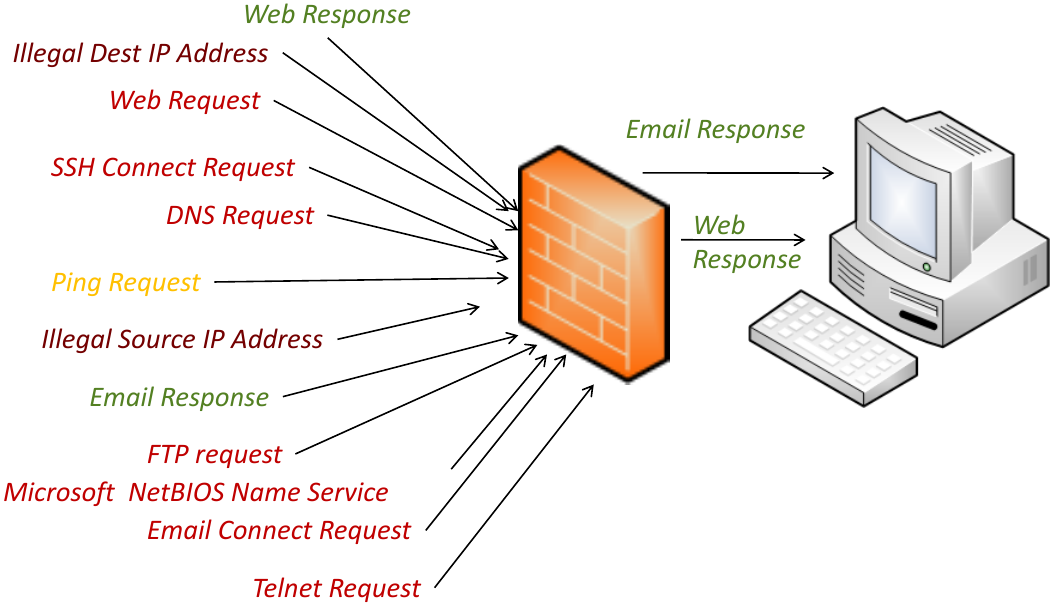
\includegraphics[scale=0.45]{packetFilterFirewall}
 \caption{Schema di funzionamento generale di un firewall filtratore di
pacchetti}
\end{figure}

\paragraph*{Multi-Homed Firewall}

Vuol dire che ci sono due uscite: una che va verso la DMZ e una verso la rete
privata.

VPN significa \textit{Virtual Private Network}, che permettono alle macchine di
essere virtualmente sulla stessa rete. Tutte le grandi società hanno una propria
VPN.

\paragraph*{Regole di sicurezza per gli accessi}

Le regole derivano innanzitutto dalle policy di sicurezza. L'altro input per
dare le regole è il mondo del reale (capacità di filtering). Dopo che le regole
sono state scritte sicuramente possiamo fare PDCA\footnote{Detto anche
\textit{Ciclo di Deming} \url{https://en.wikipedia.org/wiki/PDCA}} per
migliorare le regole. Le policy vanno aggiornate,
in base alla posizione aziendale (più o meno aggressiva) e ai breakthrough
tecnologici (es. introduzione del cloud computing).

\begin{figure}[H]
 \centering
 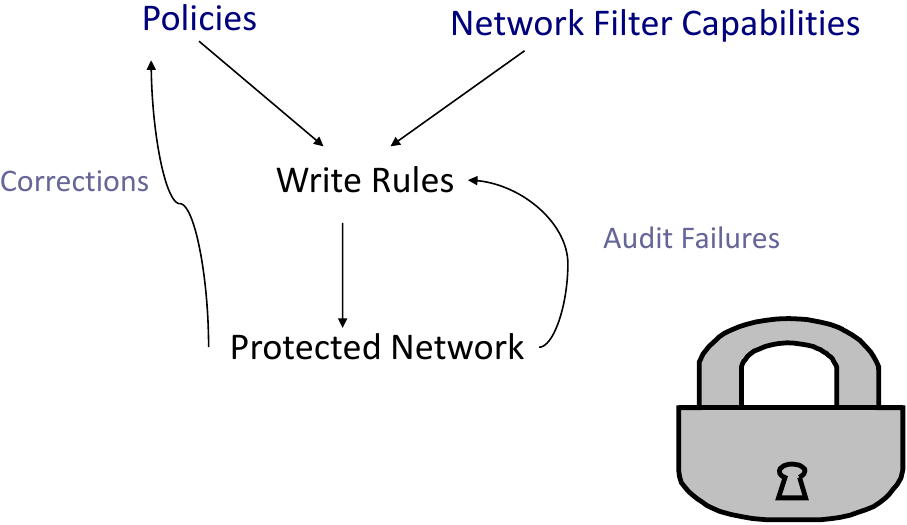
\includegraphics[scale=0.45]{writingRules}
 \caption{\textit{Flow} per la scrittura delle regole di sicurezza per gli
accessi}
\end{figure}

\subsection{Canali di accesso logico}

Sono i canali tramite i quali è possibile accedere a una rete.

Esistono diversi canali di accesso, che sono qui elencati in ordine
decrescente di pericolosità:
\begin{enumerate}
 \item USB;
 \item WLAN (la seconda più pericolosa perché vi si può accedere da fuori
l'azienda);
 \item Internet (non così pericolosa perché c'è il firewall).
\end{enumerate}

È importante quindi che anche queste entrate vengano protette.

\paragraph*{Esempio di applicazioni di una scuola}

Qui di seguito viene riportato un esempio:

\begin{table}[H]
\centering
\resizebox{\textwidth}{!}{%
\begin{tabular}{|l|p{5cm}|p{3cm}|p{3cm}|}
\hline
\textbf{Applicazioni} & \textbf{Origine} & \textbf{Server} & \textbf{Controlli
richiesti} \\
\hline
Voti; Lauree & Registrazione Universitaria & Laureati & Confidenzialità;
Integrità; Autenticazione \\
\hline
Voti; Studenti Correnti & Stati Uniti & Laureandi & Confidenzialità; Integrità;
Autenticazione \\
\hline
Pagamenti & Pagamenti internazionali; Reports Universitari & Laureandi &
Confidenzialità; Integrità; Autenticazione; Non-ripudio \\
\hline
Pagine Web & Internazionale & DMZ: aperto al pubblico & \\
\hline
\end{tabular}%
}
\caption{Un esempio di diversi canali di accesso logici per una infrastruttura
universitaria}
\end{table}

\subsection{Intrusion Detection Systems \& Intrusion Prevention Systems}

Detti anche IDS e IPS sono dei sistemi che aiutano la protezione del sistema.
Gli HIDS sono detti anche \textit{Host IDS} e sono IDS installati nella
macchina. Questi sistemi purtroppo non hanno una mappa completa del traffico di
rete, e non riescono a proteggere in maniera efficace il computer. C'è un
problema di falsi positivi da tenere conto: il sistema potrebbe individuare che
si sta facendo qualcosa di scorretto perché il comportamento devia dallo
standard, ma non è necessariamente un comportamento negativo.

\subsubsection{IDS Intelligence Systems}

Basati sulle firme: pattern specifici vengono riconosciuti come attacchi.
Problema dei falsi positivi.

Basati sulla statistica: viene capito il comportamento atteso del sistema. Se
c'è una variazione, potrebbe esserci un attacco.

Basati su reti neurali: base statistica con auto-apprendimento.

\subsubsection{Honeypot \& Honeynet}

Un \textit{honeypot} è un sistema su cui sono montati software spciali
che sembrano facili da hackerare,
mentre un l'\textit{honeynet} è una rete in cui sembra semplice accedere
e che sembra offrire del valore.   
Queste due trappole servono a catturare gli attaccanti e studiare 
i diversi tipi di attacchi\footnote{Vengono spesso utilizzate dalle
università}. Tutto il traffico che passa per questi sistemi va considerato
sospetto e deve pertanto essere attentamente monitorato.

\paragraph{Data privacy}

\begin{itemize}
\item Confidenzialità;
\item Autenticità;
\item Integrità;
\item Nonrepudation: non c'è la possibilità di dire "\textit{non l'ho inviato io
quel messaggio}" (firma digitale). Le chiavi simmetriche non garantiscono questa
proprietà e quindi non si possono implementare per fare pagamenti online.
\end{itemize}

\paragraph{Remote Access Security}

Le VPN vengono spesso implementate con IPSec.

IPSec è un protocollo di rete che permette di autenticare e criptare i
pacchetti mandati lungo la rete. Include anche protocolli per stabilire mutue
autenticazioni tra agenti all'inizio di una sessione e permette inoltre le
negoziazioni di chiavi crittografiche. IPSec permette di progettare flussi di
dati tra due host, tra due \textit{gateway} o tra un \textit{gateway} e un
host.

\paragraph{Secure Hash Functions}

L'hash è una funzione matematica che prende in input una stringa di dimensione
arbitraria e restituisce una stringa di dimensione fissa. La sicurezza di oggi è
basata sugli \textit{hash}. Presenta diverse proprietà:
\begin{itemize}
\item La non invertibilità (\emph{one way hash});
\item Collision resistance: è difficile trovare una coppia $(x_1,x_2)$ tale che
$h(x_1) = h(x_2)$ con $h$ funzione di hash\footnote{Grazie a questa proprietà si
possono eseguire le firme digitali.}.
\end{itemize}

\subparagraph*{Utilizzo}

Per utilizzare gli hash si può prendere il messaggio $M$, eseguire l'hash di $M$
($h(M)$) e appendere questo risultato alla fine, avendo quindi $payload = M +
h(M)$. A questo punto, è possibile inviare il messaggio. Il destinatario dovrà
solamente eseguire l'hash del messaggio per verificare che il messaggio sia
stato correttamente inviato.

\subparagraph*{HMAC\footnote{\url{https://it.wikipedia.org/wiki/HMAC}}}

È un RFC specifico, riconosciuto come standard e utilizzato nell'invio dei
messaggi.


\paragraph{Firma elettronica}

Come si fa a firmare un messaggio? Si prende il messaggio e lo si esponenzia
alla chiave privata. Chi lo riceve utilizza la chiave pubblica per decriptare il
messaggio. In questo modo abbiamo la non-repudiabilità.

Mandiamo una coppia $ \langle m, Sig(h(m)) \rangle $ quando mi arriva un
messaggio devo controllare che
$h(m) = h(m)$ in modo da verificare che il messaggio sia integro.
